\documentclass{article}
\title{音楽理論入門 — 音のしくみからコードまで}
\author{TeX 図書館}

\begin{document}

\section{読み方 — この本の地図と 3 つの道具}

音楽理論は「音楽のルールブック」ではありません。\textbf{「なぜこの音の並びが心地よく聞こえるのか」を説明する道具箱}です。ルールを覚えること自体に意味はなく、耳で聞こえた現象に名前を付け、再現できるようにするのが目的です。だからこの本では、必ず「まず聞こえ方、あとで名前」の順で進めます。

理論をつまずかせる原因は、ほぼ 1 つ。\textbf{「音の高さが、実は飛び飛びの目盛りになっている」ことに慣れる前に、コードやスケールの話に進んでしまう}こと。鍵盤をよく見ると、音は 12 個の段差で並んでいて、すべての音楽はこの 12 個の組み合わせから作られています。まずこの目盛りに慣れ、それから積み木(音程)と、積み木の束(コード)へ進みます。

\subsection{全 10 節の見取り図}

節の配分は次のとおりです。

\begin{enumerate}
\item 第 1 節: 読み方。方針と道具を決めます。
\item 第 2〜3 節: 音の物理と音階。12 個の目盛りを作ります。
\item 第 4 節: リズムと拍。時間の面の道具を手に入れます。
\item 第 5〜6 節: 音程とコード。積み木の束を作ります。
\item 第 7〜8 節: コード進行とマイナーキー。曲の流れを扱います。
\item 第 9 節: キーと転調。曲の地図を広げます。
\item 第 10 節: まとめと次の一歩。
\end{enumerate}

各節の終わりには\textbf{解答の指針}を置きます。答えの丸写しではなく、どの音から数えて、どの型を当てはめるかを書く欄です。まず自力で 5 分考えてから、その欄を開いてください。

\subsection{本書で最初に使う式は 1 つだけ}

音の高さは、振動の速さ(振動数、単位 Hz)で決まります。そして\textbf{振動数がちょうど 2 倍になると、同じ音に聞こえる}。これがオクターブです。ピアノの「ド」は、1 オクターブ上の「ド」のちょうど半分の振動数です。

この「2 倍の間を等しいと感じる」性質が、すべての理論の出発点です。2 倍の間を 12 個の等しい段差に分けたのが第 2 節で出てくる 12 平均律で、1 段差(半音)ごとに振動数は次の倍率になります。

\[ f = 440 \times 2^{\frac{n}{12}} \]

\( n \) は基準の音(ラ = 440 Hz)からの半音の数です。この式は覚えなくて構いません。重要なのは「半音 1 つ = 振動数で約 6 パーセントの段差」という感覚です。

\begin{quote}
\textbf{【注意】}\ 音の 3 つの要素を混同しないこと。\textbf{大きさ}は振幅(エネルギー)、\textbf{高さ}は振動数(速さ)、\textbf{音色}は波形の形(倍音の含まれ方)で決まります。バイオリンとピアノが同じ音程でも違って聞こえるのは音色の違いで、理論が扱うのは主に高さです。
\end{quote}

\textbf{解答の指針:}\ まず問題文が「高さの話」か「リズムの話」かを見分ける。高さの話なら、鍵盤の図を思い浮かべて基準の音から何段(半音いくつ)進むかを数える。リズムの話なら、拍を単位として音の長さを数える。理論の問題のほとんどは「数える」だけで解けます。式よりも、鍵盤の絵を頭に描くことが先です。

\section{音の物理 — オクターブと 12 平均律}

琴の弦やギターの弦を押さえる位置を半分にすると、同じ音が一段高い所で鳴ります。弦の長さが 2 分の 1 なら振動数は 2 倍。この「2 倍で同じ音」という耳の性質は、世界中の音楽文化で共通に使われてきました。

\subsection{2 倍の間を 12 等分する}

1 オクターブ(振動数 2 倍)の間を、\textbf{振動数の比が等しい 12 段}に分けたのが\textbf{12 平均律}です。「振動数の差」ではなく「比」で等分するのがポイントです。1 段進むごとに振動数が約 1.059 倍になり、これを 12 回掛けるとちょうど 2 倍になります。

この 1 段を\textbf{半音}、2 段を\textbf{全音}と呼びます。ピアノの鍵盤は、この 12 段をそのまま並べたものです。白鍵 7 個(ドレミファソラシ)+ 黒鍵 5 個 = 12。隣り合う鍵盤は、黒鍵を挟むかどうかに関係なく、すべて半音 1 つ違いです。

\begin{figure}
\centering
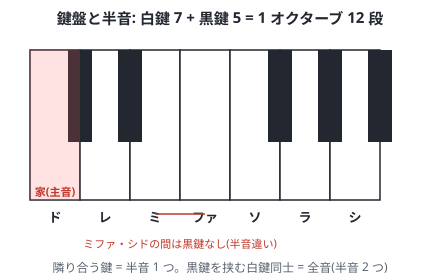
\includegraphics[width=0.9\textwidth]{figures/keyboard.svg}
\caption{鍵盤と半音: 白鍵 7 + 黒鍵 5 = 1 オクターブ 12 段}
\end{figure}

\subsection{なぜ 7 個だけ白鍵なのか}

12 段すべてを均等に使うと、旋律は覚えにくくありませんが、「どの音が家」という感覚が作りにくくなります。そこで西洋音楽は、12 段の中から\textbf{特別な 7 段}を選んで主要な席に座らせ、それをドレミファソラシドと名付けました。選び方の規則は第 3 節の主役です。

黒鍵は「白鍵の間の段差を埋める音」で、シャープ(半音上げる)とフラット(半音下げる)の印で呼びます。ドのシャープは、レのフラットと同じ鍵です(同じ音に 2 つの名前があり、曲の中でどちらの役割かで使い分けます)。

\begin{quote}
\textbf{【注意】}\ ドレミの並びには「ミファ」と「シド」の間だけ黒鍵がありません。つまりこの 2 か所はもともと半音違いです。「すべての白鍵の間に黒鍵がある」わけではない、という事実が第 3 節のスケールの設計図の核心です。
\end{quote}

\textbf{解答の指針:}\ 「音から音へ何半音か」を問う問題では、鍵盤の図に番号を振って数えます。隣の鍵なら半音 1 つ。黒鍵を飛び越えた白鍵同士は全音(半音 2 つ)。ミファとシドだけが黒鍵なしの半音違い。この 4 つの事実を書き出してから数えれば、間違いはほぼなくなります。

\section{音階 — ドレミの設計図}

ドレミファソラシドは、ただの並び順ではありません。\textbf{全音と半音が決まった順で並ぶ型}です。この型こそが\textbf{メジャースケール(長音階)}で、その構造は次の 1 行に尽きます。

\[ 全・全・半・全・全・全・半 \]

ドから始めて、レまで全音、ミまで全音、ファまで半音、ソまで全音、ラまで全音、シまで全音、上のドまで半音。ミファとシドが半音(黒鍵なし)なのは、この型に合わせて白鍵の 7 音を選んだ結果です。

\subsection{どの音から始めても同じ型}

メジャースケールの本質は「どこから始めても同じ間隔の型」です。ドから始めれば白鍵 7 音で済みますが、レから始めると型を守るために黒鍵が必要になります。例えばレから始めるメジャースケールは、レミファ\textbf{シャープ}ソラシド\textbf{シャープ}レとなり、ファとドを半音上げて型を保ちます。

これが調(キー)の正体です。\textbf{「どの音を家にして、メジャーの型を組み上げたか」}の違いであり、鍵盤上では「黒鍵をいくつ使うか」の違いとして現れます。ド(ハ)から始める調は黒鍵ゼロ、ソ(ト)から始める調はシャープ 1 つ、というように、始まりの音で使う黒鍵の数と位置が決まります。

\subsection{家の音と「ドミソ」の骨格}

スケールの中には役割の差があります。第 1 音(ド)は\textbf{主音}で、曲の帰る場所(家)です。第 5 音(ソ)は家を最も支える音(主人柱)、第 4 音(ファ)は家から外へ引っ張る音。曲が終わるときドに戻って安心するのは、この引力の働きです。

家の音の上に 3 度と 5 度を積むと、第 6 節で学ぶコードの基本形ができあがります。スケールはコードの材料表であり、コードはスケールから選んだ音の束です。この関係を押さえると、後半の内容が一気に見通せます。

\begin{quote}
\textbf{【注意】}\ 「音階は上から下へ数えるもの」ではありません。理論上は家(主音)から両方向に測ります。下のドから上のドまで数える練習は、あくまで鍵盤上の位置を掴むための訓練です。曲の中では「今の音は家から何度目か」が常に問題になります。
\end{quote}

\textbf{解答の指針:}\ 「この音から始めるメジャースケールは?」という問題では、まず全全半全全全半の型を書き、始まりの音から段差を数えていく。途中で半音が足りなければ黒鍵(シャープ)を足し、半音が飛びすぎていればフラットで戻す。最後に「ミファ・シドの半音」を型の中で見つけて照合すれば完成です。

\section{リズムと拍 — 時間の目盛り}

高さの次は時間の軸です。リズムの基本は\textbf{拍}で、心臓の鼓動のように等間隔に続く目盛りです。音の長さはすべて、この拍をいくつ占めるかで表します。

\subsection{音符の長さは 2 分割の世界}

音符の長さは、2 分の 1 を繰り返す体系になっています。

\begin{itemize}
\item 全音符: 拍 4 つ分
\item 2 分音符: 拍 2 つ分
\item 4 分音符: 拍 1 つ分
\item 8 分音符: 拍 2 分の 1(1 拍に 2 個)
\item 16 分音符: 拍 4 分の 1(1 拍に 4 個)
\end{itemize}

名前の数字は「1 拍を何分割するか」ではなく「1 小節(拍 4 つ)の中で何個で満タンか」で読むと整理しやすいです。4 分音符は 1 小節に 4 個、8 分音符なら 8 個。付点が付くと長さが 1.5 倍(元の長さ + 半分)になります。

\begin{figure}
\centering
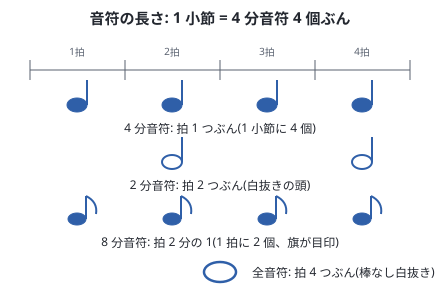
\includegraphics[width=0.9\textwidth]{figures/rhythm-notes.svg}
\caption{音符の長さと拍: 1 小節は 4 分音符 4 個ぶん}
\end{figure}

\subsection{拍子と小節}

\textbf{拍子}は、拍をいくつずつひとまとめにして数えるかの約束です。4 分の 4 拍子なら「4 分音符を単位に、4 拍で 1 小節」。3 拍子なら 3 拍で 1 小節で、ワルツの揺れはここから来ます。拍の頭(1 拍目)は\textbf{強拍}と呼ばれ、自然に力が入り、聴き手はここで曲の位置を把握します。

拍が等間隔で続くだけでは踊れません。\textbf{強弱の型}が繰り返されることで、体が次の拍を予測できるようになります。メトロノームが無味乾燥に聞こえるのは強拍がないからで、実際の演奏は拍の位置を守りつつ、強拍を少しだけ押したり引いたりしています。

\subsection{シンコペーション: 予測を裏切る技術}

拍の裏(弱い位置)にアクセントを置くことを\textbf{シンコペーション}と呼びます。聴き手の予測(頭が強い)をあえて裏切ることで、推進力やノリが生まれます。ジャズやポップスの「乗る感じ」の多くは、この裏拍の処理の工夫です。理論は「裏拍で鳴らすと予測を裏切れる」ことまでしか言えず、ノリの質は演奏文化の中で育ちます。

\begin{quote}
\textbf{【注意】}\ テンポ(速さ)と拍子(数え方)は別物です。テンポは 1 分間に何拍か(例: 120 BPM)の話で、拍子は拍をいくつで区切るかの話。同じ 4 分の 4 拍子でも、テンポ 60 とテンポ 180 では曲の性格が全く変わります。
\end{quote}

\textbf{解答の指針:}\ リズムの問題では、まず単位を拍にそろえる。1 小節 = 4 拍(4 分の 4 拍子)を基準にし、各音符が拍いくつぶんかを分数のように書き並べ、合計が 4 になるかを確認します。付点は 1.5 倍、連符は「拍を等分する」だけ。紙に拍の目盛りを引いて音を割り当てるのが、一番確実な解き方です。

\section{音程 — 音の距離の数え方}

2 つの音の高さの差を\textbf{音程}と呼びます。物理では半音の個数で測れば済みますが、音楽では\textbf{音名の数}で数える慣習(度数)を使います。ドからミまでなら、ドレミの 3 文字分で「3 度」です。混ぜないこと: 半音 4 つ = 3 度、というように両方の数え方を換算するのが理論の読み方です。

\subsection{数え方のルール}

同じ音は 1 度(ユニゾン)、隣の音名は 2 度、というように、両端を含めて数えます。だから「ドレミ」は 3 度、「ドレミファソ」は 5 度。鍵盤で半音を数えると、ドレミは半音 4 つ分(全音 2 つ)です。この「名前の数」と「半音の数」の組み合わせで、音程の性格が決まります。

\begin{itemize}
\item \textbf{長 3 度}: 半音 4 つ(ド→ミ)。明るく開く響き。
\item \textbf{短 3 度}: 半音 3 つ(ミ→ソ)。締まった、やや暗い響き。
\item \textbf{完全 5 度}: 半音 7 つ(ド→ソ)。最も安定した協和。
\item \textbf{完全 4 度}: 半音 5 つ(ド→ファ)。少し浮いた協和。
\end{itemize}

「長」「短」は半音の数の大きさ、「完全」は最も安定する組み合わせを示す伝統的な名前です。名前は後付けで、重要なのは半音の数と響きの対応です。

\subsection{協和と不協和: 振動数の比で説明できる}

2 つの音が同時に鳴るとき、振動数の比が簡単(例えば 3:2 が完全 5 度)ほど波の山と谷の重なりが規則的に戻り、耳はそれを\textbf{協和}(澄んだ響き)と感じます。比が込み入っているほど干渉が不規則になり、\textbf{不協和}(張りつめた響き)として聞こえます。

この感覚がコードの世界への入口です。不協和は「悪い音」ではなく、\textbf{次の音への引力を持つ音}です。張った音が解けるように協和へ進むと、耳は大きな満足感を得ます。曲のドラマは、この張りと解けのサイクルで作られています。

\begin{quote}
\textbf{【注意】}\ 音程は「高さの差」であって「音の良し悪し」ではありません。不協和音程は緊張を作る重要な材料です。すべて協和だけで作った曲は、静かで変化のない風景になります。
\end{quote}

\textbf{解答の指針:}\ 音程の問題では、(1) 両端を含めて名前の数を数える(例: ドファなら 4 度)、(2) 鍵盤で半音の数を数える(ドファなら 5 つ)、(3) 両方の組み合わせから長・短・完全の名前を特定する。基準音はド(またはその調の主音)に置くと形が覚えやすく、コードの第 6 節で同じ数え方がそのまま使えます。

\section{コード — 3 つの音で作る和音}

\textbf{コード(和音)}は、複数の音を同時に鳴らす束です。基本は 3 音の\textbf{トライアド(三和音)}で、家の音の上に 3 度の音を 2 つ積み上げます。

\subsection{メジャーとマイナーは積み方の違い}

ドの上に「ドミソ」を積むと\textbf{C(シー)コード}になります。構造は「下から長 3 度 + 短 3 度」(半音 4 + 3)です。この積み方を\textbf{メジャートライアド}と呼びます。

一方、「ラドミ」を積むと下から「短 3 度 + 長 3 度」(半音 3 + 4)になります。これが\textbf{マイナートライアド}で、Am(エーマイナー)と書きます。構成音の差はわずか半音 1 つ(ミとミフラットの差)なのに、響きはまったく違って聞こえます。第 6 節で詳しく扱いますが、これが「明るい/暗い」の正体です。

\begin{figure}
\centering
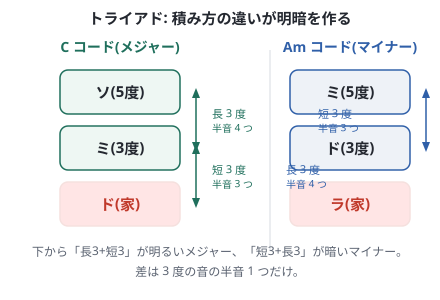
\includegraphics[width=0.9\textwidth]{figures/chord-triad.svg}
\caption{トライアド: C(メジャー)と Am(マイナー)の積み方}
\end{figure}

コード名の読み方を整理します。

\begin{itemize}
\item \textbf{C}: C(ド)を家にしたメジャートライアド。記号だけなら常にメジャー。
\item \textbf{Am}: A(ラ)を家にしたマイナートライアド。m の印がマイナーの目印。
\item \textbf{G7}: G(ソ)のメジャートライアドに、7 度の音(ファ)を追加したもの。
\end{itemize}

7 のついたコード(\textbf{セブンス})は、4 音になった分だけ不安定さ(次への引力)が増します。曲の「次に進みたい」という推進力の多くは、この 7 の音の張りが担っています。

\subsection{コードは鍵盤の絵で覚える}

理論上の数え方に加えて、鍵盤上の形で覚えると実用になります。C は白鍵の「ドミソ」、F は「ファラド」、G は「ソシレ」。\textbf{コードを 1 つずつ暗記するのではなく、「家の音 + 3 度上 + 5 度上」という作り方(レシピ)を覚える}のが長い目で見て近道です。どのキーでも同じレシピでコードが作れます。

\begin{quote}
\textbf{【注意】}\ コードは「構成音の束」であって「鳴らす順番」ではありません。ドミソを同時に鳴らしても、ドソミと分散して弾いても、同じ C コードです。分散して鳴らす形をアルペジオ(琶音)と呼びます。
\end{quote}

\textbf{解答の指針:}\ 「このコードの構成音は?」という問題では、(1) 家の音(コード名の頭文字)を鍵盤に置き、(2) メジャーかマイナーかで積み方を選ぶ(長3+短3 か 短3+長3)、(3) 3 度を 2 回積んで 3 音を書き出す。7 の付いたコードなら、さらに家から 7 度の音(メジャーなら半音 10 つ、マイナーなら半音 9 つ)を追加します。数え終わったら鍵盤の図で 3 度ずつ跳ねているか確認します。

\section{コード進行 — 曲が動く引力}

1 つのコードは静止した絵です。コードを並べて\textbf{時間的な流れ}を作ったものが\textbf{コード進行}で、曲の「物語の構造」を担います。

\subsection{主要三和音: 家・橋・引き戻し}

スケールの各音の上にコードを作ると、曲に使うコードの表ができあがります。中でも役割が大きい 3 つを主要三和音と呼びます。

\begin{itemize}
\item \textbf{I(トニック、家)}: C コード。安定の中心。ここに着地すると「終わった」感覚が生まれる。
\item \textbf{IV(サブドミナント、橋)}: F コード。家から少し外へ出る音。広がりや旅立ちの響き。
\item \textbf{V(ドミナント、引き戻し)}: G コード(特に G7)。家への引力が最も強く、鳴ったあとは C に戻りたくなる。
\end{itemize}

「C → F → G7 → C」のような進行は、\textbf{家から出て、橋を渡り、引き戻されて帰宅する}旅の構造です。聴き手はこの帰宅を予測して楽しみます。なぜ戻りたくなるのかは振動数の比で説明でき、G コードの構成音(ソシレファ)が C コードへの解決を最も促す形になっています。

\subsection{代表的な進行と「似ている」感覚}

流行の曲に繰り返し現れる進行の型があり、それぞれに通称があります。

\begin{itemize}
\item \textbf{カノン進行}(I - V - vi - IV): 弦楽の名曲の低音進行から。王道の感動系。
\item \textbf{王道進行}(IV - V - iii - vi): 力強く前に進む感覚。昭和の歌謡曲から現代まで頻出。
\item \textbf{小室進行}(vi - IV - I - V): 切なさと疾走感の同居する型。
\end{itemize}

「違う曲なのに似ている」と感じる最大の理由が、この進行の型の共有です。\textbf{メロディが違っても、進行とリズムが同じなら骨格は同じ}だからです。逆に、自分で曲を作るときは型から入るのが最短の方法になります。

\begin{quote}
\textbf{【注意】}\ 進行は「ルールで決められた正解」ではありません。I から V への引力のような\textbf{傾向}を材料に、作曲家が意図で並べています。理論は過去の名曲の傾向の記録であり、破る自由は常に作曲家にあります。ただし破ったときの効果を設計するには、破られる前の傾向を知る必要があります。
\end{quote}

\textbf{解答の指針:}\ コード進行の問題では、まず調(キー)を確定し、スケールの各音の上にコードを並べた表を作る(ドなら C Dm Em F G Am の並び)。次に問われている進行を度数(I や IV など)に翻訳して、家・橋・引き戻しのどの役割が連続しているかを読む。進行を覚えるときは度数(相対的な形)で覚え、キーが変わっても使えるようにします。

\section{マイナーキー — なぜ暗く聞こえるのか}

同じスケールから作られたコードでも、家の音を変えると曲の表情が変わります。\textbf{マイナーキー}の曲が暗く切なく聞こえる理由を、構造で説明します。

\subsection{マイナースケールの型}

メジャースケール(全全半全全全半)に対して、\textbf{ナチュラルマイナー}の型は「全・半・全・全・半・全・全」です。ラから始めれば白鍵だけで作れる(ラシドレミファソラ)ので、これは「ドのメジャースケールの家をラに移したもの」です。事実、A マイナーと C メジャーは\textbf{同じ 7 音を使う親戚}(平行調)です。

違いは家の位置だけなのに、聞こえ方が大きく変わります。理由の核心は\textbf{家のコードがマイナー(ラドミ)になる}ことです。第 6 節で見たとおり、マイナートライアドはメジャーと半音 1 つの差(3 度の音が半音低い)で、この 1 段差が「暗い」と感じる响应応のほぼすべてです。

\subsection{相对関係: 同じ音の 2 つの顔}

「同じ音の並びで、家が違うだけで表情が変わる」ことは、実用上も重要です。C メジャーの曲と A マイナーの曲は同じ音の集合を使うので、\textbf{即興で弾くときは 1 つのスケールで両方に対応できます}。ギターやピアノで「この曲のスケールは何か」を考えるとき、まず調を確定してから家(主音)を見極めるのは、このためです。

マイナーキーの主要三和音は Am(家)・Dm(橋)・E7(引き戻し)で、メジャーキーとまったく同じ「家・橋・引き戻し」の構造が、暗い色の絵の具で描かれていると考えると整理しやすいです。構造は同じ、色が違う。

\begin{quote}
\textbf{【注意】}\ 「暗い曲 = マイナーコードが多い」だけではありません。メジャーキーの曲でも、経過的にマイナーコード(Dm や Em)は普通に使われます。曲全体の明暗を決めるのは\textbf{家がメジャーかマイナーか}と、終わり方が C か Am かです。部分部分の色と全体の地の色を区別しましょう。
\end{quote}

\textbf{解答の指針:}\ 「この曲はメジャーかマイナーか」を問う問題では、(1) 使われている音を集める、(2) 候補のキー(数少ない)を当てはめる、(3) 最後のコードと、最初・途中で最も「家」らしく使われているコードを確認する。最後が Am なら A マイナー、C なら C メジャーが有力です。メロディの終音も家の音であることが多いので、併せて確認します。

\section{キーと転調 — 地図を広げる}

曲がずっと同じキーのままだと、長い曲では単調になります。\textbf{転調}は、途中で家を引っ越す技術です。引っ越し前後の対比で、曲に場面転換のような効果を生みます。

\subsection{近い調と遠い調}

すべてのキーは「黒鍵をいくつ使うか」で整理でき、鍵盤上の黒鍵の数の差が転調の距離になります。黒鍵が 1 個だけ違う調(\textbf{近親調})は、音の大部分を共有しているので、転調しても違和感がありません。例えば C メジャーから G メジャー(シャープ 1 つ)への転調は、ファの音がファシャープに変わるだけなので、滑らかです。

逆に、離れた調へ一気に転調すると強烈な「場面が変わった」感覚が得られます。サビで曲が一段明るく高揚する技法(半音上のキーへ上げる転調)は、この遠距離の引っ越しを利用した古典的な盛り上げの手段です。

\subsection{転調の実際: 引力を使って引っ越す}

うまい転調は、いきなり引っ越すのではなく\textbf{新しい家への引力}を使います。旧キーの IV 番のコードは、実は新キーの I 番(家)だった、という共通のコードを橋にするのが定石です。聴き手は同じコードを「前の家の橋」として聞いた直後、「新しい家」として聞き直すので、自然に引っ越せた感覚を得ます。

\begin{quote}
\textbf{【注意】}\ 転調は頻繁にやると効果が消えます。家を何度も変えると、聴き手はどこにも着地できず、曲全体が浮いて聞こえます。転調は曲の中で最大の「場面転換」の 1 つとして、使う位置を絞るのが基本です。
\end{quote}

\textbf{解答の指針:}\ 「この曲の転調先はどのキーか」を考える問題では、(1) 転調後に使われ始めた新しい音(旧キーにない音)を見つける、(2) その音を含む近親調を列挙する、(3) 転調後の家のコードと最後の着地から確定する。逆に「滑らかな転調にするには?」という作る側の問題では、両方のキーに共通するコード(または音)を橋に置く方針を書き出します。

\section{まとめと次の一歩}

9 節を振り返ります。道具は、実は 4 つしかありません。

\begin{itemize}
\item \textbf{12 平均律}: 鍵盤の 12 段。すべての音の材料。
\item \textbf{メジャーの型}: 全全半全全全半。家の位置がキー。
\item \textbf{度数の数え方}: 名前の数と半音の数の 2 本立て。コードのレシピに直結。
\item \textbf{家・橋・引き戻し}: I と IV と V。進行と転調はすべてこの引力の話。
\end{itemize}

理論の学習で一番効くのは、\textbf{耳と手を一緒に動かすこと}です。この本を読んだ節について、実際の音(鍵盤アプリでも可)でコードを鳴らし、その響きと名前を結びつけてください。理論は「分かった気」になりやすい科目ですが、C と Cm を実際に弾き比べた経験があるかどうかで、第 6 節の理解の質が全く変わります。

次の一歩としては、この本の先は次のような本へつながります。

\begin{itemize}
\item 音の物理をもう一度 → \textbf{高校物理やり直し}(振動と波の節がそのまま土台です)
\item 12 平均律の数学の先 → \textbf{大学数学入門}(比と指数関数が振動数を支配しています)
\item 波を分解する話の先 → \textbf{フーリエ解析入門}(あらゆる音は正弦波の重ね合わせです)
\item 耳で学ぶ習慣の作り方 → \textbf{ノートと読み書きの技法}(聴き取った音を記録する方法)
\end{itemize}

音楽理論は、耳の体験に名前を付ける科目です。名前が付いた音は、次から自分の道具として呼び出せます。まずは身近な 1 曲を「家・橋・引き戻し」で聴き直すことから始めてください。

\end{document}
